\documentclass[11pt,a4paper]{article}
\usepackage[margin=1.8cm]{geometry}
\usepackage{booktabs,pgfplots,placeins}
\usepackage[hidelinks]{hyperref}
\usepgfplotslibrary{groupplots}
\pgfplotsset{compat=1.18}
\definecolor{riderorange}{HTML}{D66B27}
\title{MNIST and CIFAR-10: native-workflow timing comparison}
\author{}\date{20 October 2026}
\makeatletter\setlength{\@fptop}{0pt}\makeatother
\newcommand{\TimingDataDir}{../../result_check/paper_version_staging/versions/v06_v15_4_full_study/generated/timing}
\begin{document}\maketitle
Non-IID, seed 42, 100 initial clients, 40\% FR3. Our v15.4 data: 100 completed rounds per dataset. STD-DAGMM: 100 completed rounds per dataset, five fresh fitting epochs each, no removals. These totals are measured, not projected. Components absent from historical logs are not estimated. Network communication was not measured. Different native trajectories, hardware load, local attacker evaluation and timer boundaries preclude a causal speedup comparison. The CIFAR detector encountered near-zero available RAM, so paging may affect its timings; paging was not measured.
\begin{table}[!ht]\centering\footnotesize
\caption{Measured STD-DAGMM component times (seconds per round, mean $\pm$ sample SD, 100 rounds per dataset).}\label{tab:std-segments}
\begin{tabular}{lrr}\toprule Component & MNIST & CIFAR-10 \\ \midrule
Client training & 33.986 $\pm$ 1.539 & 76.208 $\pm$ 4.164 \\
Simulated FR response & 0.062 $\pm$ 0.006 & 0.255 $\pm$ 0.055 \\
Server aggregation & 0.042 $\pm$ 0.004 & 0.189 $\pm$ 0.043 \\
Global evaluation & 2.144 $\pm$ 0.073 & 4.547 $\pm$ 0.227 \\
Update preparation & 0.045 $\pm$ 0.004 & 0.127 $\pm$ 0.015 \\
Detector fitting & 13.629 $\pm$ 0.467 & 45.029 $\pm$ 1.671 \\
Detector scoring & 0.278 $\pm$ 0.011 & 0.856 $\pm$ 0.035 \\
Flag decision & 0.000 $\pm$ 0.000 & 0.027 $\pm$ 0.024 \\
All detector work & 13.952 $\pm$ 0.476 & 46.040 $\pm$ 1.695 \\
Combined compute & 50.186 $\pm$ 1.943 & 127.239 $\pm$ 5.478 \\
\bottomrule\end{tabular}
\par\smallskip\begin{minipage}{0.96\textwidth}\scriptsize Our historical training, aggregation, detection and trap-generation components: not separately recorded. Network transmission: not measured in either local simulator. STD has no traps. All detector work includes preparation, fitting, scoring and decisions; it overlaps those table rows and must not be added a second time.\end{minipage}\end{table}
\begin{table}[!ht]\centering\footnotesize
\caption{Native-workflow timing over 100 executed rounds per method and dataset. All entries are measured; this is not a controlled speedup experiment.}\label{tab:timing-horizons}
\begin{tabular}{llrrr}\toprule Dataset & Workflow / horizon & Rounds & Mean s/round & Sum (min) \\ \midrule
MNIST & Ours, measured full horizon & 100 & 34.41 & 57.35 \\
MNIST & STD-DAGMM, measured full horizon & 100 & 50.19 & 83.64 \\
CIFAR-10 & Ours, measured full horizon & 100 & 84.85 & 141.41 \\
CIFAR-10 & STD-DAGMM, measured full horizon & 100 & 127.24 & 212.06 \\
\bottomrule\end{tabular}\end{table}
\begin{table}[!ht]\centering\footnotesize
\caption{Our 100 measured rounds grouped by events. Within-category mean is not detector-only overhead; amortized contribution is category sum / 100.}\label{tab:timing-phases}
\begin{tabular}{llrrr}\toprule Dataset & Round category & Count & Within-category mean (s) & Contribution (s/round) \\ \midrule
MNIST & Warm-up & 10 & 37.00 & 3.70 \\
MNIST & Probe without cycle decision & 27 & 34.29 & 9.26 \\
MNIST & Full-cycle decision & 3 & 34.45 & 1.03 \\
MNIST & Single audit & 6 & 33.95 & 2.04 \\
MNIST & Ordinary & 54 & 34.04 & 18.38 \\
CIFAR-10 & Warm-up & 10 & 117.76 & 11.78 \\
CIFAR-10 & Probe without cycle decision & 63 & 82.04 & 51.68 \\
CIFAR-10 & Full-cycle decision & 7 & 84.26 & 5.90 \\
CIFAR-10 & Single audit & 2 & 76.76 & 1.54 \\
CIFAR-10 & Ordinary & 18 & 77.51 & 13.95 \\
\bottomrule\end{tabular}\end{table}

\FloatBarrier
\clearpage
\begin{figure}[!ht]\centering\begin{tikzpicture}
\begin{groupplot}[group style={group size=2 by 1,horizontal sep=1.6cm,vertical sep=1.6cm},
width=0.43\textwidth,height=6.2cm,
grid=major,grid style={black!8},axis line style={black!35},
tick label style={font=\scriptsize},label style={font=\small},title style={font=\small},
legend style={font=\scriptsize,draw=none},scaled y ticks=false]
\nextgroupplot[title={MNIST: 100 measured rounds},ybar stacked,bar width=32pt,ymin=0,ylabel={Mean seconds per round},xtick={1,2},xticklabels={Ours,STD-DAGMM},enlarge x limits=0.7,legend to name=timing-segments-legend,legend columns=3]
\addplot[fill=blue!65!black,draw=white] table[x=x,y=honest_training_seconds] {\TimingDataDir/segments_mnist.dat};
\addlegendentry{Client training}
\addplot[fill=cyan!65!black,draw=white] table[x=x,y=fabrication_seconds] {\TimingDataDir/segments_mnist.dat};
\addlegendentry{Simulated FR response}
\addplot[fill=teal!75!black,draw=white] table[x=x,y=aggregation_seconds] {\TimingDataDir/segments_mnist.dat};
\addlegendentry{Server aggregation}
\addplot[fill=yellow!70!orange,draw=white] table[x=x,y=evaluation_seconds] {\TimingDataDir/segments_mnist.dat};
\addlegendentry{Global evaluation}
\addplot[fill=violet!70,draw=white] table[x=x,y=preparation_seconds] {\TimingDataDir/segments_mnist.dat};
\addlegendentry{Update preparation}
\addplot[fill=riderorange,draw=white] table[x=x,y=fit_seconds] {\TimingDataDir/segments_mnist.dat};
\addlegendentry{Detector fitting}
\addplot[fill=red!70!black,draw=white] table[x=x,y=score_decision_seconds] {\TimingDataDir/segments_mnist.dat};
\addlegendentry{Scoring + flag decision}
\addplot[fill=black!45,draw=white] table[x=x,y=unsegmented_seconds] {\TimingDataDir/segments_mnist.dat};
\addlegendentry{Ours: undivided round total}
\nextgroupplot[title={CIFAR-10: 100 measured rounds},ybar stacked,bar width=32pt,ymin=0,ylabel={Mean seconds per round},xtick={1,2},xticklabels={Ours,STD-DAGMM},enlarge x limits=0.7]
\addplot[fill=blue!65!black,draw=white] table[x=x,y=honest_training_seconds] {\TimingDataDir/segments_cifar10.dat};
\addplot[fill=cyan!65!black,draw=white] table[x=x,y=fabrication_seconds] {\TimingDataDir/segments_cifar10.dat};
\addplot[fill=teal!75!black,draw=white] table[x=x,y=aggregation_seconds] {\TimingDataDir/segments_cifar10.dat};
\addplot[fill=yellow!70!orange,draw=white] table[x=x,y=evaluation_seconds] {\TimingDataDir/segments_cifar10.dat};
\addplot[fill=violet!70,draw=white] table[x=x,y=preparation_seconds] {\TimingDataDir/segments_cifar10.dat};
\addplot[fill=riderorange,draw=white] table[x=x,y=fit_seconds] {\TimingDataDir/segments_cifar10.dat};
\addplot[fill=red!70!black,draw=white] table[x=x,y=score_decision_seconds] {\TimingDataDir/segments_cifar10.dat};
\addplot[fill=black!45,draw=white] table[x=x,y=unsegmented_seconds] {\TimingDataDir/segments_cifar10.dat};
\end{groupplot}\end{tikzpicture}
\par\ref{timing-segments-legend}
\caption{Mean timing over 100 executed rounds per method and dataset: non-IID FR3, seed 42, 100 initial clients, 40\% free riders. STD-DAGMM has measured task components; our gray bars are undivided whole-round totals, not zero-cost detection. Both means include rounds 1--100. Different trajectories, timer coverage and host load prevent a causal speedup claim.}\label{fig:timing-segments}
\end{figure}

\FloatBarrier
\clearpage
\begin{figure}[!ht]\centering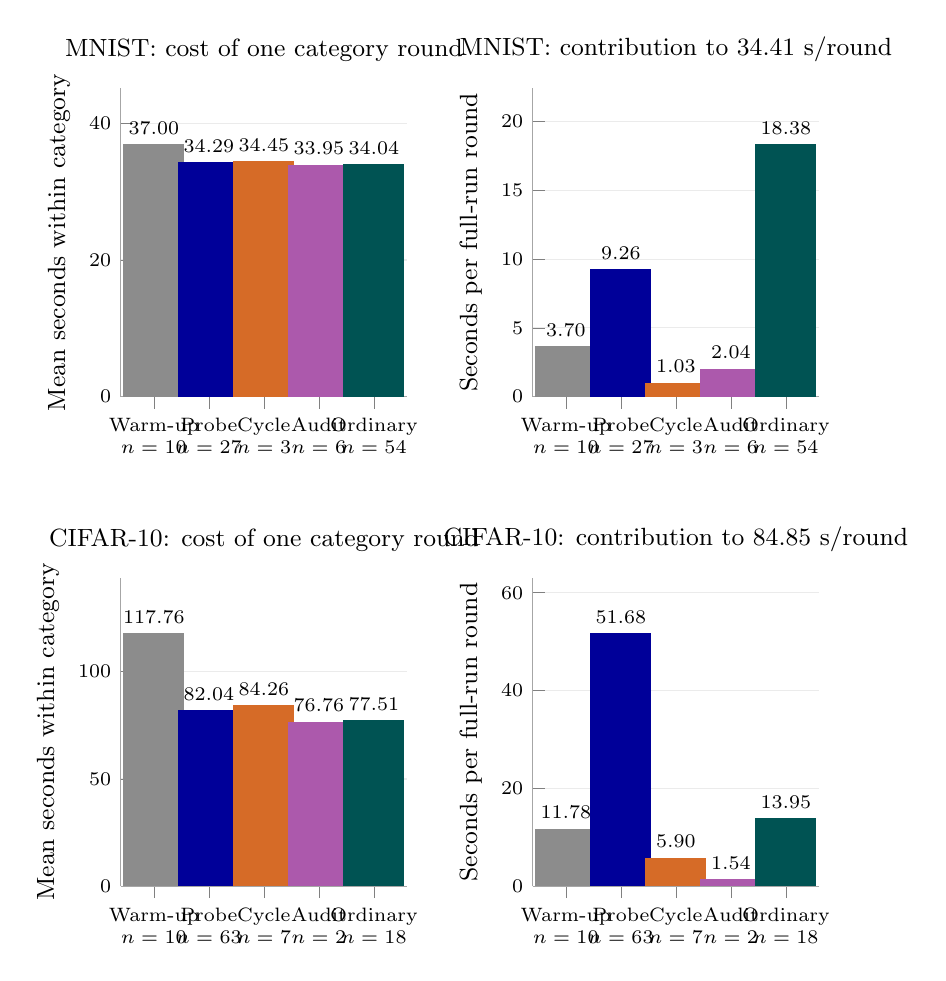
\begin{tikzpicture}
\begin{groupplot}[group style={group size=2 by 2,horizontal sep=1.6cm,vertical sep=2.3cm},
width=0.43\textwidth,height=5.5cm,
grid=major,grid style={black!8},axis line style={black!35},
tick label style={font=\scriptsize},label style={font=\small},title style={font=\small},
legend style={font=\scriptsize,draw=none},scaled y ticks=false]
\nextgroupplot[title={MNIST: cost of one category round},ybar,bar width=22pt,bar shift=0pt,ymin=0,ymax=45.135779,xmin=0.4,xmax=5.6,ylabel={Mean seconds within category},xtick={1,2,3,4,5},xticklabels={{Warm-up\\$n=10$},{Probe\\$n=27$},{Cycle\\$n=3$},{Audit\\$n=6$},{Ordinary\\$n=54$}},xticklabel style={align=center,font=\scriptsize},xmajorgrids=false,axis x line*=bottom,axis y line*=left,nodes near coords,every node near coord/.append style={font=\scriptsize,text=black,/pgf/number format/fixed,/pgf/number format/precision=2,/pgf/number format/fixed zerofill}]
\addplot[fill=black!45,draw=none,bar shift=0pt] coordinates {(1,36.996540260)};
\addplot[fill=blue!60!black,draw=none,bar shift=0pt] coordinates {(2,34.288500330)};
\addplot[fill=riderorange,draw=none,bar shift=0pt] coordinates {(3,34.450482100)};
\addplot[fill=violet!65,draw=none,bar shift=0pt] coordinates {(4,33.951632300)};
\addplot[fill=teal!65!black,draw=none,bar shift=0pt] coordinates {(5,34.036154717)};
\nextgroupplot[title={MNIST: contribution to 34.41 s/round},ybar,bar width=22pt,bar shift=0pt,ymin=0,ymax=22.423019,xmin=0.4,xmax=5.6,ylabel={Seconds per full-run round},xtick={1,2,3,4,5},xticklabels={{Warm-up\\$n=10$},{Probe\\$n=27$},{Cycle\\$n=3$},{Audit\\$n=6$},{Ordinary\\$n=54$}},xticklabel style={align=center,font=\scriptsize},xmajorgrids=false,axis x line*=bottom,axis y line*=left,nodes near coords,every node near coord/.append style={font=\scriptsize,text=black,/pgf/number format/fixed,/pgf/number format/precision=2,/pgf/number format/fixed zerofill}]
\addplot[fill=black!45,draw=none,bar shift=0pt] coordinates {(1,3.699654026)};
\addplot[fill=blue!60!black,draw=none,bar shift=0pt] coordinates {(2,9.257895089)};
\addplot[fill=riderorange,draw=none,bar shift=0pt] coordinates {(3,1.033514463)};
\addplot[fill=violet!65,draw=none,bar shift=0pt] coordinates {(4,2.037097938)};
\addplot[fill=teal!65!black,draw=none,bar shift=0pt] coordinates {(5,18.379523547)};
\nextgroupplot[title={CIFAR-10: cost of one category round},ybar,bar width=22pt,bar shift=0pt,ymin=0,ymax=143.668467,xmin=0.4,xmax=5.6,ylabel={Mean seconds within category},xtick={1,2,3,4,5},xticklabels={{Warm-up\\$n=10$},{Probe\\$n=63$},{Cycle\\$n=7$},{Audit\\$n=2$},{Ordinary\\$n=18$}},xticklabel style={align=center,font=\scriptsize},xmajorgrids=false,axis x line*=bottom,axis y line*=left,nodes near coords,every node near coord/.append style={font=\scriptsize,text=black,/pgf/number format/fixed,/pgf/number format/precision=2,/pgf/number format/fixed zerofill}]
\addplot[fill=black!45,draw=none,bar shift=0pt] coordinates {(1,117.761038190)};
\addplot[fill=blue!60!black,draw=none,bar shift=0pt] coordinates {(2,82.037953983)};
\addplot[fill=riderorange,draw=none,bar shift=0pt] coordinates {(3,84.261838643)};
\addplot[fill=violet!65,draw=none,bar shift=0pt] coordinates {(4,76.756039800)};
\addplot[fill=teal!65!black,draw=none,bar shift=0pt] coordinates {(5,77.510055911)};
\nextgroupplot[title={CIFAR-10: contribution to 84.85 s/round},ybar,bar width=22pt,bar shift=0pt,ymin=0,ymax=63.054371,xmin=0.4,xmax=5.6,ylabel={Seconds per full-run round},xtick={1,2,3,4,5},xticklabels={{Warm-up\\$n=10$},{Probe\\$n=63$},{Cycle\\$n=7$},{Audit\\$n=2$},{Ordinary\\$n=18$}},xticklabel style={align=center,font=\scriptsize},xmajorgrids=false,axis x line*=bottom,axis y line*=left,nodes near coords,every node near coord/.append style={font=\scriptsize,text=black,/pgf/number format/fixed,/pgf/number format/precision=2,/pgf/number format/fixed zerofill}]
\addplot[fill=black!45,draw=none,bar shift=0pt] coordinates {(1,11.776103819)};
\addplot[fill=blue!60!black,draw=none,bar shift=0pt] coordinates {(2,51.683911009)};
\addplot[fill=riderorange,draw=none,bar shift=0pt] coordinates {(3,5.898328705)};
\addplot[fill=violet!65,draw=none,bar shift=0pt] coordinates {(4,1.535120796)};
\addplot[fill=teal!65!black,draw=none,bar shift=0pt] coordinates {(5,13.951810064)};
\end{groupplot}\end{tikzpicture}
\caption{Where our 100-round runtime is spent (non-IID FR3, seed 42, 40\% free riders). Rows separate MNIST and CIFAR-10. Left: mean duration of a complete round in each category. Right: summed duration for that category divided by 100; the five bars add to the full-run mean printed in the title. Labels give category counts $n$. Probe excludes cycle-decision rounds; Cycle includes the final cycle decision; Audit is a single audit round. Categories are mutually exclusive. A cycle bar includes client training, aggregation and evaluation: it is NOT detector-only time. Axes scale independently; all bars start at zero.}\label{fig:timing-phases}
\end{figure}

\FloatBarrier
\clearpage
\begin{figure}[!ht]\centering\begin{tikzpicture}
\begin{groupplot}[group style={group size=2 by 1,horizontal sep=1.6cm,vertical sep=1.6cm},
width=0.43\textwidth,height=6.4cm,
grid=major,grid style={black!8},axis line style={black!35},
tick label style={font=\scriptsize},label style={font=\small},title style={font=\small},
legend style={font=\scriptsize,draw=none},scaled y ticks=false]
\nextgroupplot[title={MNIST},xmin=0,xmax=101,ymin=0,xlabel={Round},ylabel={Measured seconds},xtick={1,20,40,60,80,100},legend to name=timing-trace-legend,legend columns=3]
\addplot[black!65,thick] table[x=round,y=seconds] {\TimingDataDir/timeline_mnist.dat};
\addlegendentry{Ours: actual 100 rounds}
\addplot[only marks,mark=*,mark size=2pt,color=riderorange] table[x=round,y=seconds] {\TimingDataDir/cycle_rounds_mnist.dat};
\addlegendentry{Full-cycle decision rounds}
\addplot[blue!70!black,thick] table[x=round,y=seconds] {\TimingDataDir/std_rounds_mnist.dat};
\addlegendentry{STD: actual rounds 1--100}
\nextgroupplot[title={CIFAR-10},xmin=0,xmax=101,ymin=0,xlabel={Round},ylabel={Measured seconds},xtick={1,20,40,60,80,100}]
\addplot[black!65,thick] table[x=round,y=seconds] {\TimingDataDir/timeline_cifar10.dat};
\addplot[only marks,mark=*,mark size=2pt,color=riderorange] table[x=round,y=seconds] {\TimingDataDir/cycle_rounds_cifar10.dat};
\addplot[blue!70!black,thick] table[x=round,y=seconds] {\TimingDataDir/std_rounds_cifar10.dat};
\end{groupplot}\end{tikzpicture}
\par\ref{timing-trace-legend}
\caption{Actual per-round durations over 100 executed rounds for both methods. Our trajectories include changing active-client counts and probing schedules; STD-DAGMM retains all 100 clients. Markers indicate full-cycle decisions, not their isolated computational cost. Axis scales differ by dataset.}\label{fig:timing-traces}
\end{figure}

\FloatBarrier
\end{document}
